% Options for packages loaded elsewhere
\PassOptionsToPackage{unicode}{hyperref}
\PassOptionsToPackage{hyphens}{url}
\documentclass[
]{book}
\usepackage{xcolor}
\usepackage{amsmath,amssymb}
\setcounter{secnumdepth}{5}
\usepackage{iftex}
\ifPDFTeX
  \usepackage[T1]{fontenc}
  \usepackage[utf8]{inputenc}
  \usepackage{textcomp} % provide euro and other symbols
\else % if luatex or xetex
  \usepackage{unicode-math} % this also loads fontspec
  \defaultfontfeatures{Scale=MatchLowercase}
  \defaultfontfeatures[\rmfamily]{Ligatures=TeX,Scale=1}
\fi
\usepackage{lmodern}
\ifPDFTeX\else
  % xetex/luatex font selection
\fi
% Use upquote if available, for straight quotes in verbatim environments
\IfFileExists{upquote.sty}{\usepackage{upquote}}{}
\IfFileExists{microtype.sty}{% use microtype if available
  \usepackage[]{microtype}
  \UseMicrotypeSet[protrusion]{basicmath} % disable protrusion for tt fonts
}{}
\makeatletter
\@ifundefined{KOMAClassName}{% if non-KOMA class
  \IfFileExists{parskip.sty}{%
    \usepackage{parskip}
  }{% else
    \setlength{\parindent}{0pt}
    \setlength{\parskip}{6pt plus 2pt minus 1pt}}
}{% if KOMA class
  \KOMAoptions{parskip=half}}
\makeatother
\usepackage{color}
\usepackage{fancyvrb}
\newcommand{\VerbBar}{|}
\newcommand{\VERB}{\Verb[commandchars=\\\{\}]}
\DefineVerbatimEnvironment{Highlighting}{Verbatim}{commandchars=\\\{\}}
% Add ',fontsize=\small' for more characters per line
\usepackage{framed}
\definecolor{shadecolor}{RGB}{248,248,248}
\newenvironment{Shaded}{\begin{snugshade}}{\end{snugshade}}
\newcommand{\AlertTok}[1]{\textcolor[rgb]{0.94,0.16,0.16}{#1}}
\newcommand{\AnnotationTok}[1]{\textcolor[rgb]{0.56,0.35,0.01}{\textbf{\textit{#1}}}}
\newcommand{\AttributeTok}[1]{\textcolor[rgb]{0.13,0.29,0.53}{#1}}
\newcommand{\BaseNTok}[1]{\textcolor[rgb]{0.00,0.00,0.81}{#1}}
\newcommand{\BuiltInTok}[1]{#1}
\newcommand{\CharTok}[1]{\textcolor[rgb]{0.31,0.60,0.02}{#1}}
\newcommand{\CommentTok}[1]{\textcolor[rgb]{0.56,0.35,0.01}{\textit{#1}}}
\newcommand{\CommentVarTok}[1]{\textcolor[rgb]{0.56,0.35,0.01}{\textbf{\textit{#1}}}}
\newcommand{\ConstantTok}[1]{\textcolor[rgb]{0.56,0.35,0.01}{#1}}
\newcommand{\ControlFlowTok}[1]{\textcolor[rgb]{0.13,0.29,0.53}{\textbf{#1}}}
\newcommand{\DataTypeTok}[1]{\textcolor[rgb]{0.13,0.29,0.53}{#1}}
\newcommand{\DecValTok}[1]{\textcolor[rgb]{0.00,0.00,0.81}{#1}}
\newcommand{\DocumentationTok}[1]{\textcolor[rgb]{0.56,0.35,0.01}{\textbf{\textit{#1}}}}
\newcommand{\ErrorTok}[1]{\textcolor[rgb]{0.64,0.00,0.00}{\textbf{#1}}}
\newcommand{\ExtensionTok}[1]{#1}
\newcommand{\FloatTok}[1]{\textcolor[rgb]{0.00,0.00,0.81}{#1}}
\newcommand{\FunctionTok}[1]{\textcolor[rgb]{0.13,0.29,0.53}{\textbf{#1}}}
\newcommand{\ImportTok}[1]{#1}
\newcommand{\InformationTok}[1]{\textcolor[rgb]{0.56,0.35,0.01}{\textbf{\textit{#1}}}}
\newcommand{\KeywordTok}[1]{\textcolor[rgb]{0.13,0.29,0.53}{\textbf{#1}}}
\newcommand{\NormalTok}[1]{#1}
\newcommand{\OperatorTok}[1]{\textcolor[rgb]{0.81,0.36,0.00}{\textbf{#1}}}
\newcommand{\OtherTok}[1]{\textcolor[rgb]{0.56,0.35,0.01}{#1}}
\newcommand{\PreprocessorTok}[1]{\textcolor[rgb]{0.56,0.35,0.01}{\textit{#1}}}
\newcommand{\RegionMarkerTok}[1]{#1}
\newcommand{\SpecialCharTok}[1]{\textcolor[rgb]{0.81,0.36,0.00}{\textbf{#1}}}
\newcommand{\SpecialStringTok}[1]{\textcolor[rgb]{0.31,0.60,0.02}{#1}}
\newcommand{\StringTok}[1]{\textcolor[rgb]{0.31,0.60,0.02}{#1}}
\newcommand{\VariableTok}[1]{\textcolor[rgb]{0.00,0.00,0.00}{#1}}
\newcommand{\VerbatimStringTok}[1]{\textcolor[rgb]{0.31,0.60,0.02}{#1}}
\newcommand{\WarningTok}[1]{\textcolor[rgb]{0.56,0.35,0.01}{\textbf{\textit{#1}}}}
\usepackage{longtable,booktabs,array}
\usepackage{calc} % for calculating minipage widths
% Correct order of tables after \paragraph or \subparagraph
\usepackage{etoolbox}
\makeatletter
\patchcmd\longtable{\par}{\if@noskipsec\mbox{}\fi\par}{}{}
\makeatother
% Allow footnotes in longtable head/foot
\IfFileExists{footnotehyper.sty}{\usepackage{footnotehyper}}{\usepackage{footnote}}
\makesavenoteenv{longtable}
\usepackage{graphicx}
\makeatletter
\newsavebox\pandoc@box
\newcommand*\pandocbounded[1]{% scales image to fit in text height/width
  \sbox\pandoc@box{#1}%
  \Gscale@div\@tempa{\textheight}{\dimexpr\ht\pandoc@box+\dp\pandoc@box\relax}%
  \Gscale@div\@tempb{\linewidth}{\wd\pandoc@box}%
  \ifdim\@tempb\p@<\@tempa\p@\let\@tempa\@tempb\fi% select the smaller of both
  \ifdim\@tempa\p@<\p@\scalebox{\@tempa}{\usebox\pandoc@box}%
  \else\usebox{\pandoc@box}%
  \fi%
}
% Set default figure placement to htbp
\def\fps@figure{htbp}
\makeatother
\setlength{\emergencystretch}{3em} % prevent overfull lines
\providecommand{\tightlist}{%
  \setlength{\itemsep}{0pt}\setlength{\parskip}{0pt}}
\usepackage[]{natbib}
\bibliographystyle{plainnat}
\usepackage{booktabs}
\usepackage{bookmark}
\IfFileExists{xurl.sty}{\usepackage{xurl}}{} % add URL line breaks if available
\urlstyle{same}
\hypersetup{
  pdftitle={Forecasting},
  pdfauthor={Samuel Rowe adapted from Wooldridge (2011)},
  hidelinks,
  pdfcreator={LaTeX via pandoc}}

\title{Forecasting}
\author{Samuel Rowe adapted from Wooldridge (2011)}
\date{2025-09-20}

\begin{document}
\maketitle

{
\setcounter{tocdepth}{1}
\tableofcontents
}
\begin{Shaded}
\begin{Highlighting}[]
\NormalTok{bookdown}\SpecialCharTok{::}\FunctionTok{render\_book}\NormalTok{()}
\end{Highlighting}
\end{Shaded}

\chapter*{Overview}\label{overview}
\addcontentsline{toc}{chapter}{Overview}

\begin{enumerate}
\def\labelenumi{\arabic{enumi}.}
\tightlist
\item
  Preparing for Forecasting
\item
  Forecasting and Comparing Models
\end{enumerate}

\chapter{Prepare for Forecasting}\label{prepare-for-forecasting}

\section{Graph the Time Series}\label{graph-the-time-series}

We'll use our Phillip's Curve data to forecast unemployment one-step into the future

Set Time Series

\begin{Shaded}
\begin{Highlighting}[]
\NormalTok{cd }\StringTok{"/Users/Sam/Desktop/Econ 645/Data/Wooldridge"}
\KeywordTok{use}\NormalTok{ phillips.dta, }\KeywordTok{clear}
\KeywordTok{tsset} \FunctionTok{year}
\end{Highlighting}
\end{Shaded}

\begin{verbatim}
/Users/Sam/Desktop/Econ 645/Data/Wooldridge

        time variable:  year, 1948 to 2003
                delta:  1 unit
\end{verbatim}

Use \emph{tsline} command to graph the time series

\begin{Shaded}
\begin{Highlighting}[]
\KeywordTok{tsline}\NormalTok{ inf}
\KeywordTok{graph} \KeywordTok{export} \StringTok{"/Users/Sam/Desktop/Econ 645/Stata/week\_11\_inflation.png"}\NormalTok{, }\KeywordTok{replace}
\end{Highlighting}
\end{Shaded}

\begin{figure}
\centering
\pandocbounded{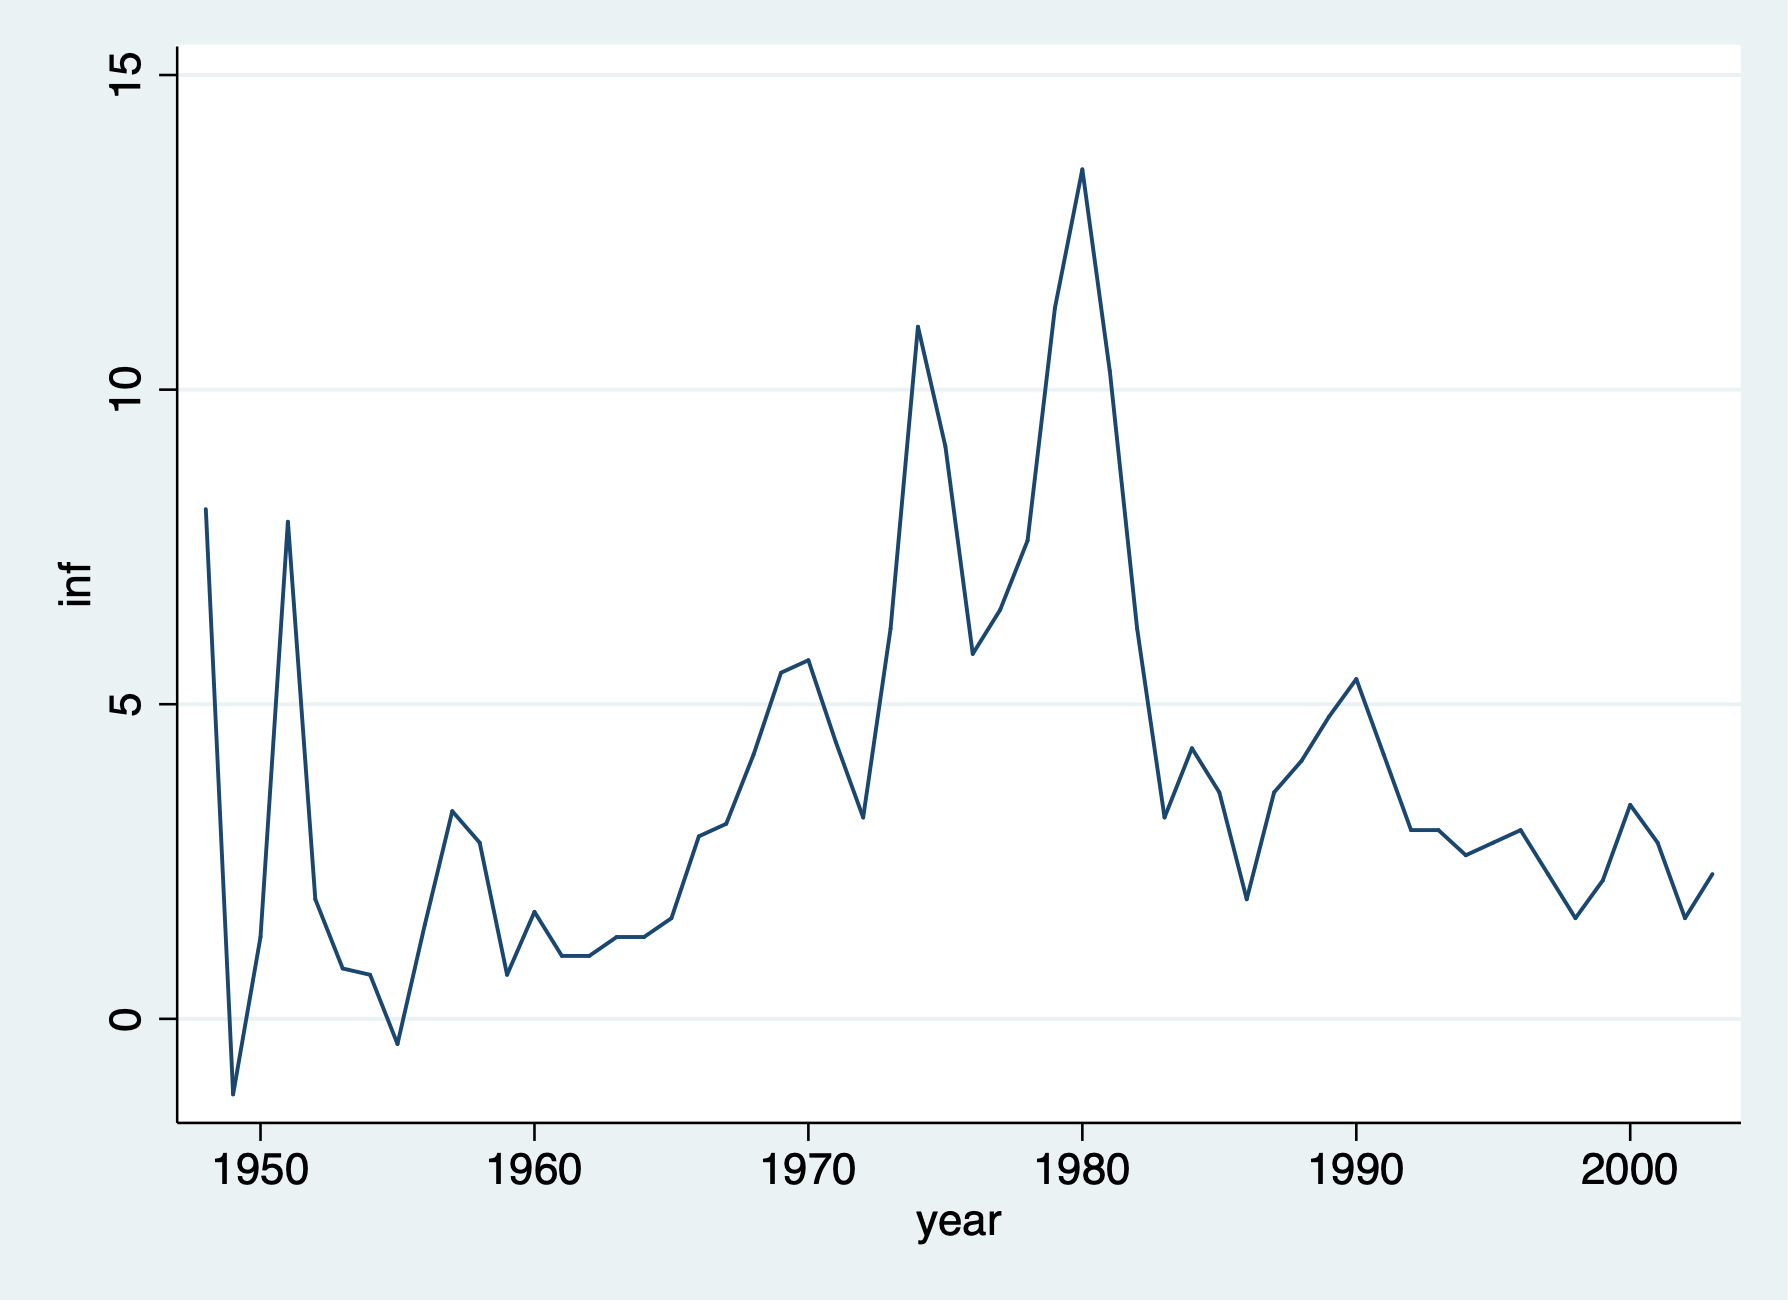
\includegraphics[keepaspectratio]{week_11_inflation.png}}
\caption{Graph of Inflation Rate}
\end{figure}

\section{Train and Test}\label{train-and-test}

First we need to Generate training and test samples, so we'll use the time
series sequence until 1996 as our training data, and we'll use 1997 to 2003
as our testing data.

\begin{Shaded}
\begin{Highlighting}[]
\KeywordTok{gen} \KeywordTok{test}\NormalTok{ = 0}
\KeywordTok{replace} \KeywordTok{test}\NormalTok{ = 1 }\KeywordTok{if} \FunctionTok{year}\NormalTok{ \textgreater{}= 1997}
\KeywordTok{label} \KeywordTok{define}\NormalTok{ test1 0 }\StringTok{"training sample"}\NormalTok{ 1 }\StringTok{"testing sample"}
\KeywordTok{label} \KeywordTok{values} \KeywordTok{test}\NormalTok{ test1}
\OtherTok{list} \FunctionTok{year}\NormalTok{ unem inf }\KeywordTok{test}
\end{Highlighting}
\end{Shaded}

\begin{verbatim}
(7 real changes made)

     +-------------------------------------------------+
     | year        unem          inf              test |
     |-------------------------------------------------|
  1. | 1948         3.8    8.1000004   training sample |
  2. | 1949   5.9000001         -1.2   training sample |
  3. | 1950   5.3000002          1.3   training sample |
  4. | 1951         3.3    7.9000001   training sample |
  5. | 1952           3          1.9   training sample |
     |-------------------------------------------------|
  6. | 1953   2.9000001    .80000001   training sample |
  7. | 1954         5.5    .69999999   training sample |
  8. | 1955   4.4000001   -.40000001   training sample |
  9. | 1956   4.0999999          1.5   training sample |
 10. | 1957   4.3000002          3.3   training sample |
     |-------------------------------------------------|
 11. | 1958   6.8000002          2.8   training sample |
 12. | 1959         5.5    .69999999   training sample |
 13. | 1960         5.5          1.7   training sample |
 14. | 1961   6.6999998            1   training sample |
 15. | 1962         5.5            1   training sample |
     |-------------------------------------------------|
 16. | 1963   5.6999998          1.3   training sample |
 17. | 1964   5.1999998          1.3   training sample |
 18. | 1965         4.5          1.6   training sample |
 19. | 1966         3.8    2.9000001   training sample |
 20. | 1967         3.8    3.0999999   training sample |
     |-------------------------------------------------|
 21. | 1968   3.5999999    4.1999998   training sample |
 22. | 1969         3.5          5.5   training sample |
 23. | 1970   4.9000001    5.6999998   training sample |
 24. | 1971   5.9000001    4.4000001   training sample |
 25. | 1972   5.5999999          3.2   training sample |
     |-------------------------------------------------|
 26. | 1973   4.9000001    6.1999998   training sample |
 27. | 1974   5.5999999           11   training sample |
 28. | 1975         8.5    9.1000004   training sample |
 29. | 1976   7.6999998    5.8000002   training sample |
 30. | 1977   7.0999999          6.5   training sample |
     |-------------------------------------------------|
 31. | 1978   6.0999999    7.5999999   training sample |
 32. | 1979   5.8000002         11.3   training sample |
 33. | 1980   7.0999999         13.5   training sample |
 34. | 1981   7.5999999         10.3   training sample |
 35. | 1982   9.6999998    6.1999998   training sample |
     |-------------------------------------------------|
 36. | 1983   9.6000004          3.2   training sample |
 37. | 1984         7.5    4.3000002   training sample |
 38. | 1985   7.1999998    3.5999999   training sample |
 39. | 1986           7          1.9   training sample |
 40. | 1987   6.1999998    3.5999999   training sample |
     |-------------------------------------------------|
 41. | 1988         5.5    4.0999999   training sample |
 42. | 1989   5.3000002    4.8000002   training sample |
 43. | 1990   5.5999999    5.4000001   training sample |
 44. | 1991   6.8000002    4.1999998   training sample |
 45. | 1992         7.5            3   training sample |
     |-------------------------------------------------|
 46. | 1993   6.9000001            3   training sample |
 47. | 1994   6.0999999    2.5999999   training sample |
 48. | 1995   5.5999999          2.8   training sample |
 49. | 1996   5.4000001            3   training sample |
 50. | 1997   4.9000001          2.3    testing sample |
     |-------------------------------------------------|
 51. | 1998         4.5          1.6    testing sample |
 52. | 1999   4.1999998          2.2    testing sample |
 53. | 2000           4    3.4000001    testing sample |
 54. | 2001   4.8000002          2.8    testing sample |
 55. | 2002   5.8000002          1.6    testing sample |
     |-------------------------------------------------|
 56. | 2003           6          2.3    testing sample |
     +-------------------------------------------------+
\end{verbatim}

\section{AR(1) and VAR models}\label{ar1-and-var-models}

We'll use two models to forecast unemployment:

\begin{enumerate}
\def\labelenumi{\arabic{enumi}.}
\tightlist
\item
  AR(1) model: Just a 1-year lag of unemployment
\item
  VAR model: 1-year lag of unemployment and 1-year lag of inflation
\end{enumerate}

Run the regressions using training data

\subsection*{OLS AR-1}\label{ols-ar-1}
\addcontentsline{toc}{subsection}{OLS AR-1}

Run the model with a 1-year lag in unemployment

\begin{Shaded}
\begin{Highlighting}[]
\KeywordTok{reg}\NormalTok{ unem }\OtherTok{l}\NormalTok{.unem }\KeywordTok{if} \KeywordTok{test}\NormalTok{ == 0}
\end{Highlighting}
\end{Shaded}

\begin{verbatim}
      Source |       SS           df       MS      Number of obs   =        48
-------------+----------------------------------   F(1, 46)        =     57.13
       Model |  62.8162728         1  62.8162728   Prob > F        =    0.0000
    Residual |  50.5768515        46  1.09949677   R-squared       =    0.5540
-------------+----------------------------------   Adj R-squared   =    0.5443
       Total |  113.393124        47  2.41261967   Root MSE        =    1.0486

------------------------------------------------------------------------------
        unem |      Coef.   Std. Err.      t    P>|t|     [95% Conf. Interval]
-------------+----------------------------------------------------------------
        unem |
         L1. |   .7323538   .0968906     7.56   0.000      .537323    .9273845
             |
       _cons |   1.571741   .5771181     2.72   0.009     .4100629     2.73342
------------------------------------------------------------------------------
\end{verbatim}

\subsection*{VAR}\label{var}
\addcontentsline{toc}{subsection}{VAR}

We will add a 1-year lag in inflation along with our 1-year lag in unemployment

\begin{Shaded}
\begin{Highlighting}[]
\KeywordTok{reg}\NormalTok{ unem }\OtherTok{l}\NormalTok{.unem }\OtherTok{l}\NormalTok{.inf }\KeywordTok{if} \KeywordTok{test}\NormalTok{ == 0}
\end{Highlighting}
\end{Shaded}

\begin{verbatim}
      Source |       SS           df       MS      Number of obs   =        48
-------------+----------------------------------   F(2, 45)        =     50.22
       Model |  78.3083336         2  39.1541668   Prob > F        =    0.0000
    Residual |  35.0847907        45  .779662015   R-squared       =    0.6906
-------------+----------------------------------   Adj R-squared   =    0.6768
       Total |  113.393124        47  2.41261967   Root MSE        =    .88298

------------------------------------------------------------------------------
        unem |      Coef.   Std. Err.      t    P>|t|     [95% Conf. Interval]
-------------+----------------------------------------------------------------
        unem |
         L1. |   .6470261   .0838056     7.72   0.000     .4782329    .8158192
             |
         inf |
         L1. |   .1835766   .0411828     4.46   0.000     .1006302    .2665231
             |
       _cons |   1.303797   .4896861     2.66   0.011     .3175188    2.290076
------------------------------------------------------------------------------
\end{verbatim}

\chapter{Forecasting}\label{forecasting}

\section{One-Step Ahead Model vs Dynamic AR(1) Model}\label{one-step-ahead-model-vs-dynamic-ar1-model}

One-step ahead we can use predict or forecast for AR(1). We use the \emph{estimates store} command to store our results for our AR(1) model.

\subsection*{Train the model}\label{train-the-model}
\addcontentsline{toc}{subsection}{Train the model}

\begin{Shaded}
\begin{Highlighting}[]
\KeywordTok{reg}\NormalTok{ unem }\OtherTok{l}\NormalTok{.unem }\KeywordTok{if} \KeywordTok{test}\NormalTok{ == 0}
\KeywordTok{estimates} \KeywordTok{store}\NormalTok{ model1}
\end{Highlighting}
\end{Shaded}

\subsection*{One-Step Ahead Model}\label{one-step-ahead-model}
\addcontentsline{toc}{subsection}{One-Step Ahead Model}

We can get one-step ahead just using predict

\begin{Shaded}
\begin{Highlighting}[]
\KeywordTok{predict}\NormalTok{ unem\_est}
\end{Highlighting}
\end{Shaded}

Forecast - One-step-ahead forecast. We three addition commands:

\begin{enumerate}
\def\labelenumi{\arabic{enumi}.}
\tightlist
\item
  \emph{forecast create}
\item
  \emph{forecast estimates}
\item
  \emph{forecast solve}
\end{enumerate}

\begin{Shaded}
\begin{Highlighting}[]
\NormalTok{forecast create forecast1, }\KeywordTok{replace}
\NormalTok{forecast }\KeywordTok{estimates}\NormalTok{ model1}
\end{Highlighting}
\end{Shaded}

For a one-step ahead forecast, \textbf{static} is our key option otherwise it will not be a one-step ahead forecast.

\begin{Shaded}
\begin{Highlighting}[]
\NormalTok{forecast solve, }\KeywordTok{prefix}\NormalTok{(st\_) }\KeywordTok{begin}\NormalTok{(1997) }\KeywordTok{end}\NormalTok{(2003) }\KeywordTok{static}
\OtherTok{list} \FunctionTok{year}\NormalTok{ unem st\_unem }\KeywordTok{if} \FunctionTok{year}\NormalTok{ \textgreater{} 1996}
\end{Highlighting}
\end{Shaded}

\begin{verbatim}
Computing static forecasts for model forecast1.
-----------------------------------------------
Starting period:  1997
Ending period:    2003
Forecast prefix:  st_

1997:  .............
1998:  .............
1999:  ..............
2000:  ..............
2001:  ..............
2002:  .............
2003:  ............

Forecast 1 variable spanning 7 periods.
---------------------------------------

     +------------------------------+
     | year        unem     st_unem |
     |------------------------------|
 50. | 1997   4.9000001   5.5264521 |
 51. | 1998         4.5    5.160275 |
 52. | 1999   4.1999998   4.8673334 |
 53. | 2000           4   4.6476274 |
 54. | 2001   4.8000002   4.5011568 |
     |------------------------------|
 55. | 2002   5.8000002   5.0870399 |
 56. | 2003           6   5.8193936 |
     +------------------------------+
\end{verbatim}

\subsection*{Dynamic Model}\label{dynamic-model}
\addcontentsline{toc}{subsection}{Dynamic Model}

Dynamic model - We won't use l.unem but l.dy\_unem

\begin{Shaded}
\begin{Highlighting}[]
\NormalTok{forecast solve, }\KeywordTok{prefix}\NormalTok{(dy\_) }\KeywordTok{begin}\NormalTok{(1997) }\KeywordTok{end}\NormalTok{(2003)}
\OtherTok{list} \FunctionTok{year}\NormalTok{ unem st\_unem dy\_unem }\KeywordTok{if} \FunctionTok{year}\NormalTok{ \textgreater{} 1996}
\end{Highlighting}
\end{Shaded}

\begin{verbatim}
Computing dynamic forecasts for model forecast1.
------------------------------------------------
Starting period:  1997
Ending period:    2003
Forecast prefix:  dy_

1997:  .............
1998:  .............
1999:  ............
2000:  ............
2001:  ............
2002:  ............
2003:  ............

Forecast 1 variable spanning 7 periods.
---------------------------------------

     +------------------------------------------+
     | year        unem     st_unem     dy_unem |
     |------------------------------------------|
 50. | 1997   4.9000001   5.5264521   5.5264521 |
 51. | 1998         4.5    5.160275   5.6190596 |
 52. | 1999   4.1999998   4.8673334   5.6868811 |
 53. | 2000           4   4.6476274   5.7365503 |
 54. | 2001   4.8000002   4.5011568   5.7729259 |
     |------------------------------------------|
 55. | 2002   5.8000002   5.0870399   5.7995653 |
 56. | 2003           6   5.8193936   5.8190751 |
     +------------------------------------------+
\end{verbatim}

\subsection*{Graph Model}\label{graph-model}
\addcontentsline{toc}{subsection}{Graph Model}

Graph Actual, One-Step-Ahead Model, and Dynamic Model

\begin{Shaded}
\begin{Highlighting}[]
\KeywordTok{twoway} \KeywordTok{line}\NormalTok{ unem }\FunctionTok{year}\NormalTok{ || }\KeywordTok{line}\NormalTok{ st\_unem }\FunctionTok{year}\NormalTok{, lpattern(}\KeywordTok{dash}\NormalTok{) || }\KeywordTok{line}\NormalTok{ dy\_unem }\FunctionTok{year}\NormalTok{, lpattern(}\BaseNTok{dot}\NormalTok{)}
\KeywordTok{graph} \KeywordTok{export} \StringTok{"/Users/Sam/Desktop/Econ 645/Stata/week\_11\_static\_v\_dynamic.png"}\NormalTok{, }\KeywordTok{replace}
\end{Highlighting}
\end{Shaded}

\begin{figure}
\centering
\pandocbounded{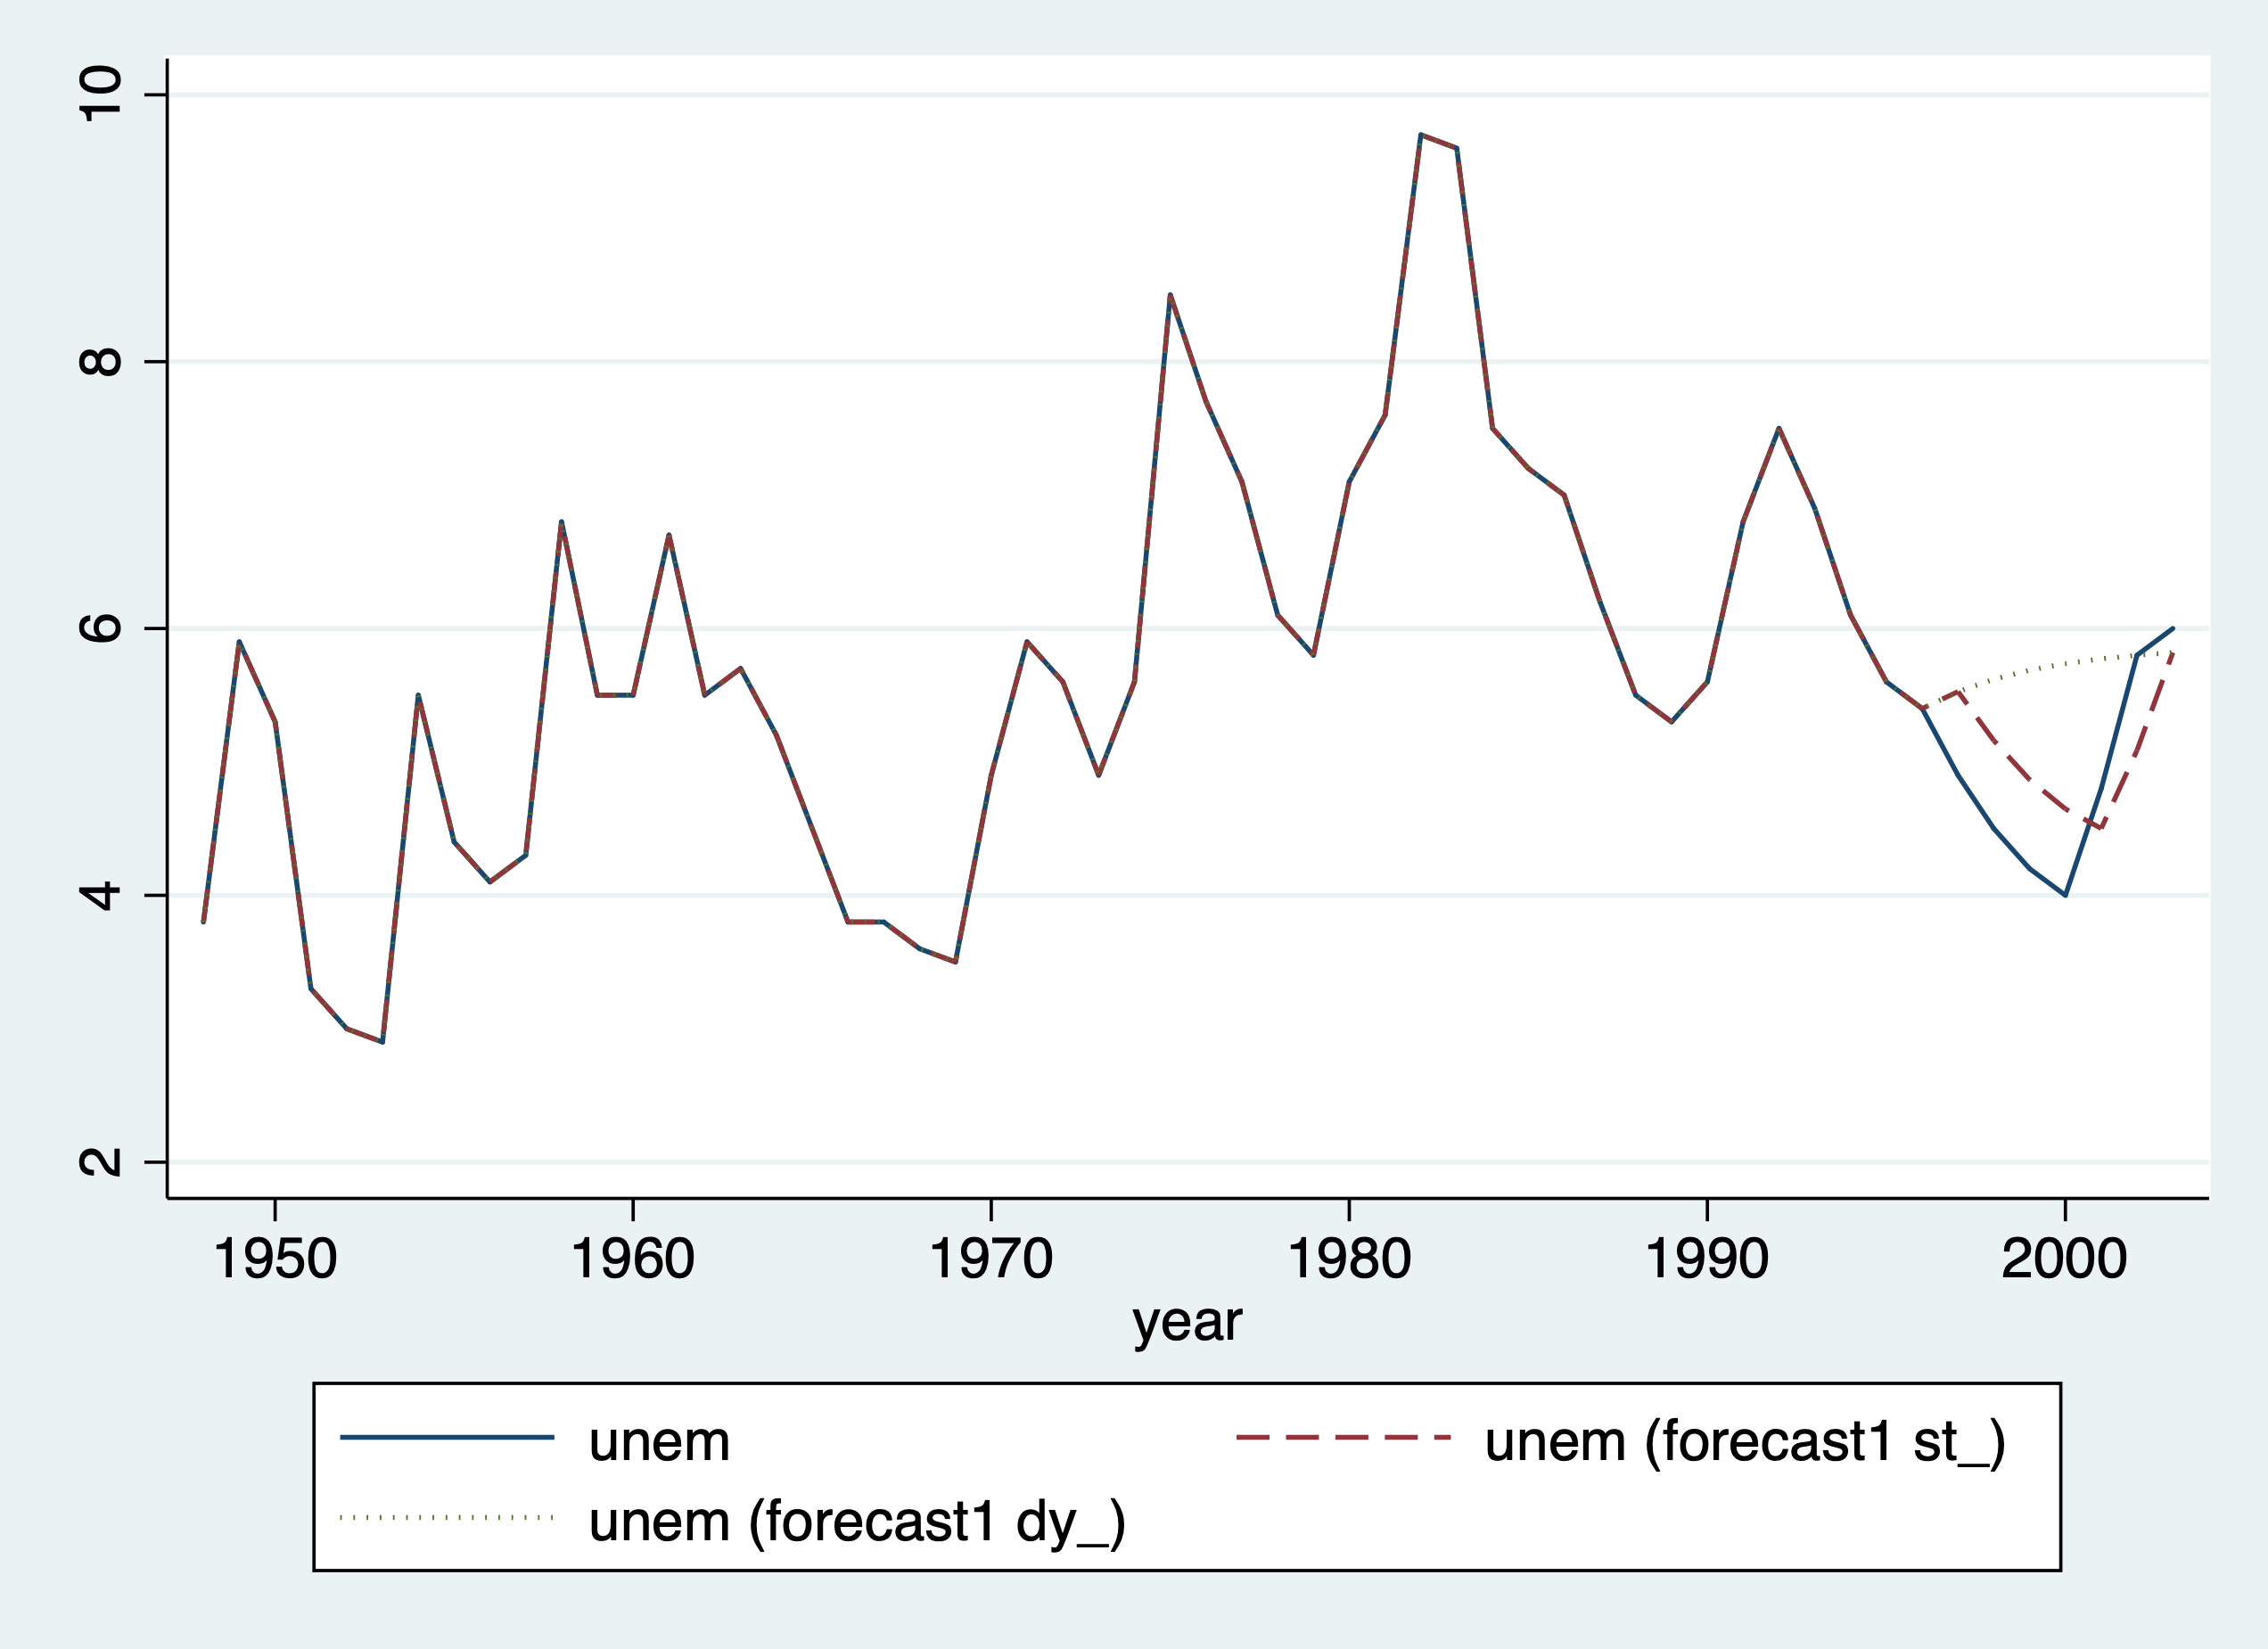
\includegraphics[keepaspectratio]{week_11_static_v_dynamic.png}}
\caption{One-Step-Ahead vs Dynamic Forecasting}
\end{figure}

\subsection*{Root Mean Squared Error (RMSE)}\label{root-mean-squared-error-rmse}
\addcontentsline{toc}{subsection}{Root Mean Squared Error (RMSE)}

Calculate RMSE for AR(1) model

\begin{Shaded}
\begin{Highlighting}[]
\KeywordTok{gen} \FunctionTok{e}\NormalTok{ = unem {-} st\_unem}
\KeywordTok{gen}\NormalTok{ e2 = }\FunctionTok{e}\NormalTok{\^{}2}
\KeywordTok{sum}\NormalTok{ e2 }\KeywordTok{if} \KeywordTok{test}\NormalTok{==1}
\FunctionTok{scalar}\NormalTok{ esum= }\OtherTok{\textasciigrave{}r(sum)\textquotesingle{}}\NormalTok{/}\OtherTok{\textasciigrave{}r(N)\textquotesingle{}}
\FunctionTok{scalar}\NormalTok{ model1\_RMSE= esum\^{}.5}
\KeywordTok{display}\NormalTok{ model1\_RMSE}
\end{Highlighting}
\end{Shaded}

\begin{verbatim}
    Variable |        Obs        Mean    Std. Dev.       Min        Max
-------------+---------------------------------------------------------
          e2 |          7    .3319141    .1891047   .0326187   .5083123



.57611988
\end{verbatim}

\subsection*{Mean Absolute Error (MAE)}\label{mean-absolute-error-mae}
\addcontentsline{toc}{subsection}{Mean Absolute Error (MAE)}

Calculate MAE for AR(1) model

\begin{Shaded}
\begin{Highlighting}[]
\NormalTok{gen e\_abs = abs(e) if test ==1}
\NormalTok{sum e\_abs if test==1}
\NormalTok{scalar model1\_MAE=\textasciigrave{}r(mean)\textquotesingle{}}
\NormalTok{display model1\_MAE}
\end{Highlighting}
\end{Shaded}

\begin{verbatim}
(49 missing values generated)

    Variable |        Obs        Mean    Std. Dev.       Min        Max
-------------+---------------------------------------------------------
       e_abs |          7     .542014    .2109284   .1806064   .7129602


.54201399
\end{verbatim}

\section{One-Step Ahead VAR Model}\label{one-step-ahead-var-model}

One-step ahead we can use predict or forecast for VAR Model (lagged employment and lagged inflation)

\subsection*{Train the Model}\label{train-the-model-1}
\addcontentsline{toc}{subsection}{Train the Model}

\begin{Shaded}
\begin{Highlighting}[]
\KeywordTok{quietly} \KeywordTok{reg}\NormalTok{ unem }\OtherTok{l}\NormalTok{.unem }\OtherTok{l}\NormalTok{.inf }\KeywordTok{if} \FunctionTok{year}\NormalTok{ \textless{} 1997}
\end{Highlighting}
\end{Shaded}

Our predict command will produce the same results as \emph{forecast solve, static}

\begin{Shaded}
\begin{Highlighting}[]
\KeywordTok{predict}\NormalTok{ p2}
\KeywordTok{estimates} \KeywordTok{store}\NormalTok{ model2}
\end{Highlighting}
\end{Shaded}

Forecast for Model 2

\begin{Shaded}
\begin{Highlighting}[]
\NormalTok{forecast create forecast2, }\KeywordTok{replace}
\NormalTok{forecast }\KeywordTok{estimates}\NormalTok{ model2}
\end{Highlighting}
\end{Shaded}

\subsection*{One-Step-Ahead Forecast of VAR Model}\label{one-step-ahead-forecast-of-var-model}
\addcontentsline{toc}{subsection}{One-Step-Ahead Forecast of VAR Model}

\begin{Shaded}
\begin{Highlighting}[]
\NormalTok{forecast solve, }\KeywordTok{prefix}\NormalTok{(st2\_) }\KeywordTok{begin}\NormalTok{(1997) }\KeywordTok{end}\NormalTok{(2003) }\KeywordTok{static}
\OtherTok{list} \FunctionTok{year}\NormalTok{ unem st\_unem }\KeywordTok{if} \FunctionTok{year}\NormalTok{ \textgreater{} 1996}
\end{Highlighting}
\end{Shaded}

\begin{verbatim}
Computing static forecasts for model forecast2.
-----------------------------------------------
Starting period:  1997
Ending period:    2003
Forecast prefix:  st2_

1997:  ............
1998:  ...........
1999:  ...........
2000:  .............
2001:  ..............
2002:  .............
2003:  ..............

Forecast 1 variable spanning 7 periods.
---------------------------------------

     +------------------------------+
     | year        unem    st2_unem |
     |------------------------------|
 50. | 1997   4.9000001   5.3484678 |
 51. | 1998         4.5    4.896451 |
 52. | 1999   4.1999998   4.5091372 |
 53. | 2000           4   4.4251752 |
 54. | 2001   4.8000002   4.5160618 |
     |------------------------------|
 55. | 2002   5.8000002   4.9235368 |
 56. | 2003           6   5.3502712 |
     +------------------------------+
\end{verbatim}

\subsection*{Dynamic Forecast of VAR Model}\label{dynamic-forecast-of-var-model}
\addcontentsline{toc}{subsection}{Dynamic Forecast of VAR Model}

\begin{Shaded}
\begin{Highlighting}[]
\NormalTok{forecast solve, }\KeywordTok{prefix}\NormalTok{(dy2\_) }\KeywordTok{begin}\NormalTok{(1997) }\KeywordTok{end}\NormalTok{(2003) }
\OtherTok{list} \FunctionTok{year}\NormalTok{ unem st2\_unem dy2\_unem }\KeywordTok{if} \FunctionTok{year}\NormalTok{ \textgreater{} 1996}
\end{Highlighting}
\end{Shaded}

\begin{verbatim}
Computing dynamic forecasts for model forecast2.
------------------------------------------------
Starting period:  1997
Ending period:    2003
Forecast prefix:  dy2_

1997:  ............
1998:  .............
1999:  .............
2000:  ............
2001:  .............
2002:  ............
2003:  .............

Forecast 1 variable spanning 7 periods.
---------------------------------------

     +------------------------------------------+
     | year        unem    st2_unem    dy2_unem |
     |------------------------------------------|
 50. | 1997   4.9000001   5.3484678   5.3484678 |
 51. | 1998         4.5    4.896451   5.1866217 |
 52. | 1999   4.1999998   4.5091372   4.9533992 |
 53. | 2000           4   4.4251752   4.9126439 |
 54. | 2001   4.8000002   4.5160618   5.1065664 |
     |------------------------------------------|
 55. | 2002   5.8000002   4.9235368   5.1218934 |
 56. | 2003           6   5.3502712   4.9115181 |
     +------------------------------------------+
\end{verbatim}

\subsection{Calculate RMSE and MAE}\label{calculate-rmse-and-mae}

Calculate RMSE for the VAR model

\begin{Shaded}
\begin{Highlighting}[]
\KeywordTok{gen} \FunctionTok{e}\NormalTok{ = unem {-} st2\_unem}
\KeywordTok{gen}\NormalTok{ e2 = }\FunctionTok{e}\NormalTok{\^{}2}
\KeywordTok{sum}\NormalTok{ e2 }\KeywordTok{if} \KeywordTok{test}\NormalTok{==1}
\FunctionTok{scalar}\NormalTok{ esum2 = }\OtherTok{\textasciigrave{}r(sum)\textquotesingle{}}\NormalTok{/}\OtherTok{\textasciigrave{}r(N)\textquotesingle{}}
\FunctionTok{scalar}\NormalTok{ model2\_RMSE=esum2\^{}.5}
\KeywordTok{display}\NormalTok{ model2\_RMSE}
\end{Highlighting}
\end{Shaded}

\begin{verbatim}
    Variable |        Obs        Mean    Std. Dev.       Min        Max
-------------+---------------------------------------------------------
          e2 |          7    .2722276    .2459784    .080621   .7681881



.52175434
\end{verbatim}

Calculate MAE for VAR model

\begin{Shaded}
\begin{Highlighting}[]
\KeywordTok{gen}\NormalTok{ e\_abs = }\FunctionTok{abs}\NormalTok{(}\FunctionTok{e}\NormalTok{)}
\KeywordTok{sum}\NormalTok{ e\_abs }\KeywordTok{if} \KeywordTok{test}\NormalTok{==1}
\FunctionTok{scalar}\NormalTok{ model2\_MAE=}\OtherTok{\textasciigrave{}r(mean)\textquotesingle{}}
\KeywordTok{display}\NormalTok{ model2\_MAE}
\end{Highlighting}
\end{Shaded}

\begin{verbatim}
    Variable |        Obs        Mean    Std. Dev.       Min        Max
-------------+---------------------------------------------------------
       e_abs |          7    .4841946    .2099534   .2839384   .8764634


.48419455
\end{verbatim}

\section{Compare AR(1) and VAR models}\label{compare-ar1-and-var-models}

Which model do we use? The model that minimizes the error.

\subsection*{Compare Results with RMSE and MSE}\label{compare-results-with-rmse-and-mse}
\addcontentsline{toc}{subsection}{Compare Results with RMSE and MSE}

\begin{Shaded}
\begin{Highlighting}[]
\KeywordTok{display} \StringTok{"Model 1: RMSE="}\NormalTok{model1\_RMSE }\StringTok{" and MAE="}\NormalTok{model1\_MAE}
\KeywordTok{display} \StringTok{"Model 2: RMSE="}\NormalTok{model2\_RMSE }\StringTok{" and MAE="}\NormalTok{model1\_MAE}
\KeywordTok{display} \StringTok{"Model 2 with lagged unemployment and lagged inflation has lower RMSE and MAE."}
\end{Highlighting}
\end{Shaded}

\begin{verbatim}
Model 1: RMSE=.57611988 and MAE=.54201399

Model 2: RMSE=.52175434 and MAE=.48419455

Model 2 with lagged unemployment and lagged inflation has lower RMSE and MAE.
\end{verbatim}

\subsection*{Graph the Forecasts}\label{graph-the-forecasts}
\addcontentsline{toc}{subsection}{Graph the Forecasts}

Forecasting Line

\begin{Shaded}
\begin{Highlighting}[]
    \KeywordTok{twoway} \KeywordTok{line}\NormalTok{ unem }\FunctionTok{year}\NormalTok{ || }\KeywordTok{line}\NormalTok{ st\_unem }\FunctionTok{year}\NormalTok{, lpattern(}\KeywordTok{dash}\NormalTok{) || }\KeywordTok{line}\NormalTok{ st2\_unem }\FunctionTok{year}\NormalTok{, lpattern(}\BaseNTok{dot}\NormalTok{) }\CommentTok{///}
    \BaseNTok{title}\NormalTok{(}\StringTok{"Forecast of Unemployment"}\NormalTok{) }\BaseNTok{xtitle}\NormalTok{(}\StringTok{"Year"}\NormalTok{) }\BaseNTok{subtitle}\NormalTok{(}\StringTok{"One{-}Step{-}Ahead"}\NormalTok{) }\BaseNTok{ytitle}\NormalTok{(}\StringTok{"Unemployment Rate"}\NormalTok{) }\BaseNTok{xline}\NormalTok{(1996) }\CommentTok{///}
    \BaseNTok{legend}\NormalTok{(}\KeywordTok{order}\NormalTok{(1 }\StringTok{"Actual"}\NormalTok{ 2 }\StringTok{"Model 1"}\NormalTok{ 3 }\StringTok{"Model 2"}\NormalTok{))}
    \KeywordTok{graph} \KeywordTok{export} \StringTok{"/Users/Sam/Desktop/Econ 645/Stata/week\_11\_forecast.png"}\NormalTok{, }\KeywordTok{replace}
\end{Highlighting}
\end{Shaded}

\begin{figure}
\centering
\pandocbounded{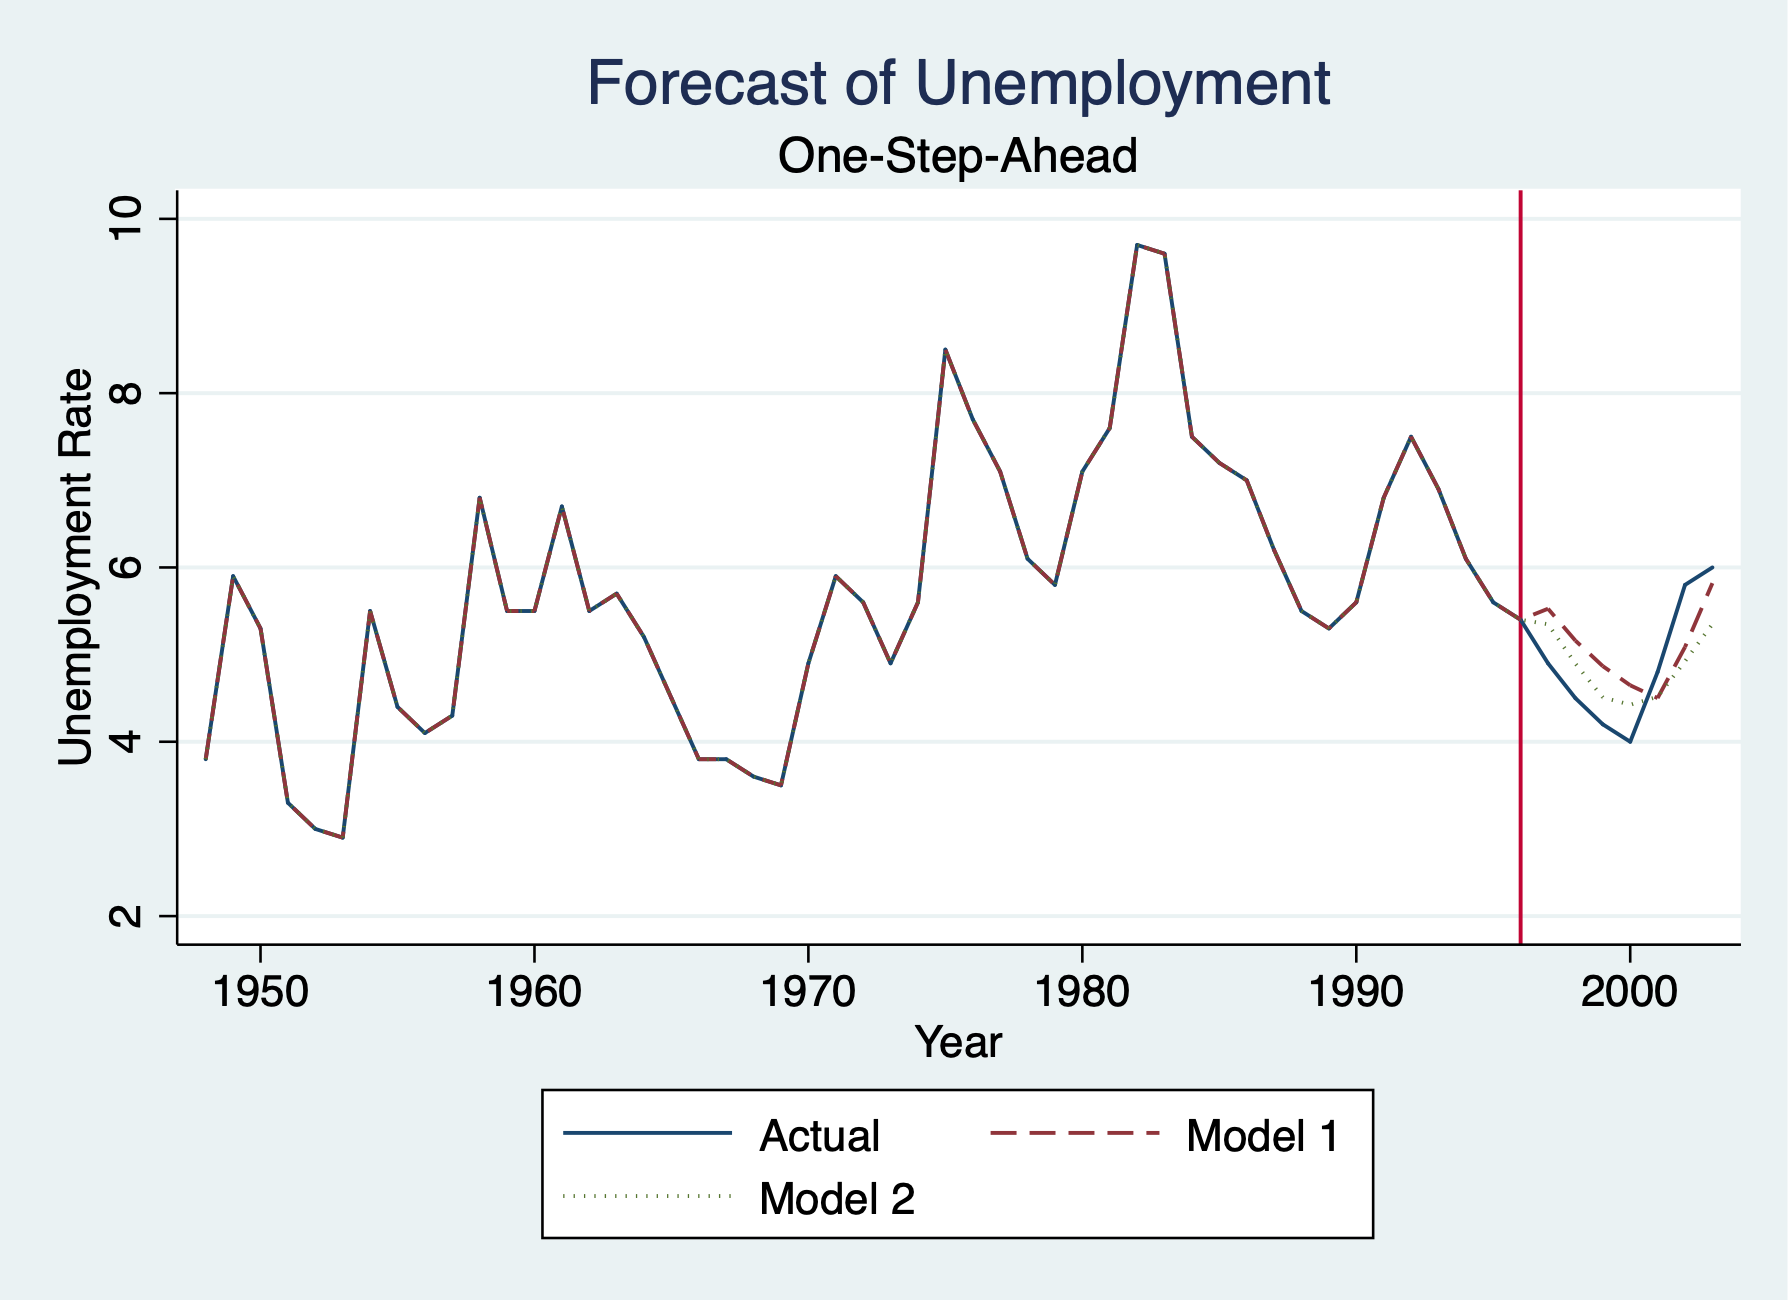
\includegraphics[keepaspectratio]{week_11_forecast.png}}
\caption{Compare Forecasts}
\end{figure}

Mitchell, N.M. (2020). \emph{Data Management Using Stata: A Practical Handbook}. (2nd ed.). Stata Press.

UCLA Advanced Research Computing. (2025). \emph{How can I access information stored after I run a command in Stata.} Retrieved from \url{https://stats.oarc.ucla.edu/stata/faq/how-can-i-access-information-stored-after-i-run-a-command-in-stata-returned-results/}

Wooldridge (2009). \emph{Introductory Econometrics: A Modern Approach}. (4th ed.). South-Western Cengage Learning.

\bibliography{book.bib,packages.bib}

\end{document}
